\clearpage
\appendix
\begingroup
\renewcommand{\chaptername}{Phụ lục}
\titleformat{\chapter}[hang]{\normalfont\bfseries\Large}{\chaptername\ \thechapter.}{0.5em}{}
\titlespacing*{\chapter}{0pt}{0pt}{12pt}
\addtocontents{toc}{\protect\renewcommand{\protect\cftchappresnum}{Phụ lục~}}
\begin{landscape}
\chapter{Sơ đồ tổng hợp quy trình RC-Free}
\label{app:master-pipeline}
\begin{figure}[H]
\centering
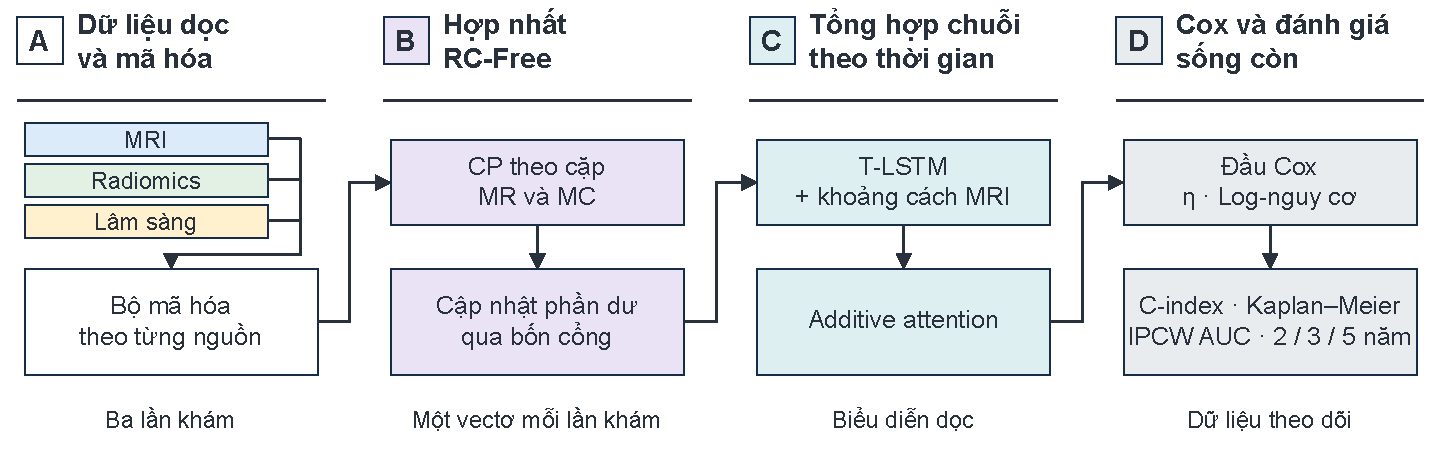
\includegraphics[width=\linewidth,height=11.5cm,keepaspectratio]{image/master-pipeline.pdf}
\caption[Quy trình RC-Free từ đầu vào đến đánh giá]{Mô hình mã hóa dữ liệu của ba lần khám theo từng nguồn (A), tính tương tác MR và MC để cập nhật biểu diễn qua các nhánh phần dư (B), rồi tổng hợp chuỗi theo thời gian (C). Khối Cox tạo điểm log-nguy cơ dùng trong đánh giá sống còn (D).}
\label{fig:master-pipeline}
\end{figure}
\end{landscape}
\endgroup
